\documentclass[11pt,oneside]{amsart}
\usepackage{alttpreamble}
% \usepackage{tocloft}
% \renewcommand{\cftsecleader}{\cftdotfill{\cftdotsep}}
\begin{document}
\author{Maya Basu}


\address{University of California, Berkeley}
\email{mab@berkeley.edu}



\title{Journal of the Resident Sparkle Squid}
\maketitle





\subsection{June 17th} The main question is can we come up with an algorithm to assign heights? One homework question was to do this for an example, and to make the inequalities work trivially, I jokingly set one of the Reeb heights to $10^8$. This is what was my eventual inspiration for how we could assign heights. My idea was that there were certain chords which could be made arbitrarily big which allowed other choords to be anything, and we would still get positive area loops. I realized this corresponded to, geometrically, stretching out the outside loops so that generators in that area were "solved" automatically. 

Then I had the next realization - by "solving" loops, I freed them up to "solve" more loops, and so I could propagate through the knot. 
We spent the rest of the day refining our understanding of exactly how the algorithm would work. 



\subsection{June 19th} Maybe the algorithm stops and doesn't end up propagating through the entire knot - in this case we shouldn't get a solution for every knot. I spent a lot of time trying to rearange knots - putting the interesections in some sort of grid and drawing the knot lines between them - to get some way to prove that the algorithm would finish. My hypothesis was that since the algorithm shouldn't necessarily work for every set of inequalities, it must be some geometric feature of the knot. Essentially, I figured because it was one long strand, this must make some restictions of the inequalities present which would help solve the problem.

We found some interesting relations based on the fact that only certain numbers of + or - generators can show up in teh inequalities, however, these wer ultimitly unhelpful.

Finally, I realized that what I was trying to do - rearrange a knot in a controlled manner was actually already a thing! I realized I could use plat position. From here, it seems very possible to complete the proof, and I eventually figured out one way to do it.


\subsection{June 21/22nd}

The biggest question next seemed to be the issue of contractible chords. As Ethan pointed out, all of the chords in the extras category were contractible, however, we found that intruducing a stabilization gave us a contractible chord in the second class. At first I was confused about why this loop would be contractible when the side loops in the trefoil were not, but then thinking about the issue algebraically, and clarifying a possible definition of contractibility, which I added to the main log, it became imediatly obvious why this was true. 

This is also when we realized the difference between contractible and super-contractible. The discussion can up while trying to go from the categories given by the algorithm to an actual height assignment. The plan was to give all contractible chords of height one, but this made very clear the issue that some contractible chords required modifying others to let them shrink - only the extras, the super contractible chords, could all necessarily be made arbitrarily small. 

Wednesday evening I started on python code to go from the plat position representation of a knot to height assignments using what we had decided to call the flooding algorith.


\subsection{June 22nd}

Finished the code! This took most of the day. 

Additionally, we discussed out next steps. It seems like to start generating visuals we should try to compute the barcode of many knots. Only finding the homology would leave out information about the basis of generators, but if we found the generators at each step of the filteration, we could easily recover the homology afterwards.


\subsection{June 23rd}

Wrote code that identifies all cycles up to a certain height, given the height filteration and the differentials. Hopefully this will help us create visuals and understand persistance better




\subsection{June 25th}

Today was mostly grinding examples, all three of us tried varying height assignments(basically the effect of a planar isotopy) and found that this just moved bars but didn't actually change the number of bars or their status as finite/infinite. 

Additionally, I started code that computes the persistant homology given the differentials, the grading, and the height assignments. While this will pribably be useful to help us check our work, my end goal is to have code that can automatically compute the barcode of any given knot, given the differentials, grading, and height assignments. This requires tracking the generators, however I have a plan of how to do this. Because I already wrote something that more or less looks for cycles, I can usilize this at each step of the persistance. That I know the persistant homology (I wil be calculating the kernel/image of each map between gradings) will tell me how many things to look for, which I think will make my task easier. For example, if I know that the kernel of a certain map from grading 1 to 0 has a certain dimentional kernel, then I know how many independent cycles to look for. I shouldn't technically need to compute the homology first, but this gives me a sanity check, and a way to write the code more iterativly, which I think I need since this is a fairly complex procedure.





\subsection{June 26th}

I suppose that this belongs is Sunday, since I finished at about 12:30 am, but I did the majority of the code for the homolgy computitions, as at 10:30 pm about, my brain decided that it was inspired, and that I absolutly couldnt call asleep untill I coded out my ideas.  ... lol.  Anyway, today was basically the same as Saturday with all of us doing examples, except Ethan worked out barcode changes for the first riedemister move, and both of them pointed out I needed to be doing computations in mod 2 for the homology code. Something isn't working quite right, but this isn't our first priority, so I will stop working on this for now. Additionally, Ethan and I spent a while trying some simple knots trying to get move three to work, but the results couldn't me augmented. 

\subsection{June 26th}

Our focus today was reidemister moves 2 and three. We started out optimisitally trying these moves on the checanov to see what happened but we ran into issues. First, It does not appear that you can even do reidemister move three on the chechanov. I spent a while trying to come up with the plat positions of various knots that might host move three, but I couldn't find a single one that was also augmentable. This is clearly going to be an issue. Fredrick was trying to do reidemister move two and eventually we all ended up working on the example. It seemed like we got the promising result that only a single finite bar was added to $H_{-1}$, but then when computing the last step in persistance, the dimentions stopped working out. Something was wrong and after trying to figure out what for a while we gave up. 

After taking a break, I realized that we shouldn't actually have to try examples, or even find examples to figure out what happened to the bars. If we could find how the DGA transformed directly then possibly we could infer changes to the barcode directly from this. I tried this with the three point move and found a morphism of the differentials that corresponded. It seemed like none of the disks changes except in very controlled ways. THis was great! Then all three of use came up with an argument for a left reidemister two move (a left cusp moving through a vertical strand) which gives us confirmation of a very simple transformation of barcodes. However, returning back to move 3, I couldnt find a way to relate the transformation of the differentials to a transformation of the bars of the barcode. This will be a goal for tommorow. 



\subsection{June 28}

Previously we were hard pressed to find a simple and valid knot which we could preform reidemister move three on, however Ethan realized that in plat position, actually we can do move three on the chekanov knot. We we calculated the persistant homology before and after doing this move. The results were not good, so much changed it was very difficult to identify how things have changed. This was very disheartening since it gave a counter example to many of the things we had guess might possibly be invariant. 

However, this gave me an idea. It seemed like the issue here was the choice of height assignment. The longer I thought about it the more convinced I was that I should try to find a height assignment that was invariant under moves three and two. This way, after a move three was done, the height assignments wouldn't change, and any change in the barcode would be due to the actual geometry of the reidemister move alone. The problem at the moment was that after the reidemister move, we had reassigned heights, and now that the generators came in a different ordwer in plat position, a bunch of the area loops, and thus the inequalites, and thus the height assignments were changed. 

So, what I wanted was an assigment of heights that didn't change the area inequalities after the move was done. By considering all possible area loops contacting a three point move, I realized that for a triangle with $+a$ and $-b$ and $-c$ in the interior of the three point move, the substitution $a = b+c$ would leave every single area calculation exactly the same! This seemed incredibly helpful. Basically, my plan was to shrink the area triangle inside of a three point move down to $\epsilon$ so that the area inequality became $a - b - c= \epsilon$. Then, after the substitution $a = b + c + \epsilon$, every other area inequality would change on the order of $\epsilon$. But, heres the great part, for every area inequality that wasn't a triangle, I would force the inequality to be something like $>>$, for example, I could require that the minimum height of a reeb chord is $1$, and that each area patch is at least $1$ unit in area (except the triangles which would be $\epsilon$). This is completly valid, and the proof of which is simply the process of the flooding algorithm which assignes heights. After the diagram is flooded, making each area loop as large as you want can be carried out by an iterative process. 


So essentially my plan was to planar isotopy a knot into another set of height assignments where every area loop with three generators is as small as possible, and every area loop with more than three generators has a significantly larger area (so that the inequalities woulnd't be disturbed byt he substitution involved in move three). On second thought, I realised that for a loop with on positibe generator and one negative generator I might want to shrink this also to prevent difficulties with riedemister move three.



As an example, I decided to try to work out a set of height inequalities for the chekanov. This was extremly difficult, as I needed to satisfy not only the overall tier strucure of the area inequalities but also the fact that equations with three generators had to be precisly satisfied. I tried this for quite literally a few hours and eventually gave up to eat dinner. Later that night I realized that instead of treating the three generator inequalities as inequalities, maybe setting them equal to say an $\epsilon_i$ and substituting into the remaining equations might be helpful. 


\subsection{June 29}

Today, I realized that I was overlooking a huge problem in my idea. What happens after the riedemister move is done, and some of the area loops contacting it how have one less generator in them? This meant that a loop that was previously large because it had four generators was now large but only had three generators though in order to continue doing moves with out a change of height assigments. This meant that in order to continue doing reidemester moves Id have to continually reassign heights in between to colapse all of the new triangles cerated. While this wouldn't be nearly as arbitrary as the process of reassigning heights essentially right to left in plat position it still sounds extremely difficult. 


Then I realized that I was being extremely dumb  - I could easily consider contracting one triangle at a time and it would work out just fine. This is the idea I developed further and realised this allows you to take the same height assignment from before as after the move - a common point of the set of valid heights.

\subsection{June 30, July 1st and 2nd}

We got distracted persuing the new definition of h-conductibility for the rest of the weekend. Tentative results from this are in log 3.0 (currently the most recent log)


\subsection{July 3rd}

We've gone back to consider how heights change very carefully to see if and how conductibility is preserved under reidemister moves. Discussing what happens during the three point move (which by no means obviously preserves the set of all valid heights because of the subtraction of the center triangle implies that we only necceserally have matching on the regieme where the triangle is smaller than the surrounding triangles). But fredrick found this paper: https://arxiv.org/pdf/math/0407347.pdf which lists conditions for doing reidemister moves in the lagrangian projection. One of those conditions is that the knot can be lagrangian isotoped so that the area of the triangle is smaller than the areas of the surrounding triangles. Now, while legrangian isotopy might change the actual hights, it doesn't change the set of height inequalities, since it doesn't change or create intesections. 



\subsection{July 5th}


We basically just did examples of trying to keep the area the same during a Reidemeister move. The tricky thing is that you can't just change the height of the strand involved in moving as it may not be possible to resolve the remaining inequalities. For example, in the knot ($4, 3, 2, 3, 2, 4$) looking to the left side of the knot, we see that in trying to preseve the total area after we move to $4,2,3,2,2,4$ by just changing generators such as $a_1$, $a_2$, $a_3$ or even $a_5$ (mathematica generator lable convention) it is not possible to get the total area unchanged (doing so would make a reeb height negative). This provides a counter example to my hope that we could control the "flow" of "area" through the knot in some predictable manner to keep the area the same before and after the move. Perhaps this is still possible but it would have to be through a much more complex process then just letting the area flow into the next adjacent areas. Additionally, I found a somewhat minimal area for ($4, 3, 2, 3, 2, 4$ ) by going backwards in the algorithm - basically my method was to first find the tiers, then collect all equations in which only generators in the last tier appear as negative (which exist by definition) and find heights (every height is an integer, every area is at least one) to satisfy those minimally etc. Then you can move up a tier untill all generators are determined. This finds a "local minima" of sorts but we dont know that this is the global minima. Then I remembered something I read about on stack overflow before, and realized that this was exactly in the format that a linear programing thingy would solve  - $ax + b \ge 0 $ and a set of constraints. Fredrick and Ethan got this working on mathematica and we confirmed that the global minimum of area for this knot is the same as I found by hand (though I have no reason to believe that in general this is true or feasible to do by hand). 


\subsection{July 6th}

Today I made the executive decision that the knot which has been so useful to us many times ($4, 3, 2, 3, 2, 4$) is officially the Platypus knot. We used the platypus knot to test out minimizing area and seeing what happens in various cases. Unfortunatly the barcode of the knot seems to change quite a bit still, so anything that is invariant in this case is more subtle then we have guessed so far. The area restriction is very interesting - trying to manipulate the knot so that the area remains unchanged is supprisingly difficult. I was confused yesterday why I couldn't get a valid height assigment for after reidemister move three on the knot untill I eventualy reallized that it is just not possible to do the move with the "cannonical"(area minimizing) height assignemnts in place (because the area of the triangle is larger than some of the sourrounding areas). 





\subsection{July 10th}


We tried to see how the flooding algorithm interacts with reidemister moves to see how we could modify it in order to possibly work better with the moves. In the end, one generator switched up a tier, if this is possible we could potentially have absolutly no order preserved (all possible orderings could be created by composing this and it's inverse) but this is just a worst case senario this might not actually happen.



I wanted to see how reidemister move two interacts with large loops and this is what I came up with: Consider a large loop with many positives and negatives that gets split, via move two, into two loops. This move two introduces a positive into one of these loops and a negative into the other loop. Call the new crossing which introduces the negative into a loop $a$ and the other crossing $b$, which introduces a positive into the other half of the split loop. Then we know that for this to be a valid reidemeister move two, there must be at least on other positive in the loop with $a$. Now we first notice that if we keep $|a - b|$ to be small (say $\epsilon$) then the surrounding areas outside are modified by at most $\epsilon$.This means we only have to worry about what happens to the two loops that the initial loop split into. 

There are two cases, either there is no positive (other than $b$) in the loop not containing $a$, and when there are one or more positives in this loop. First we consider the case when there is no other positive, meaning we have a loop with only $b$ as positive. 

Consider how the flooding algorithm works, assuming that islands don't exist (the algorithm always terminates) we know that the negative crossings in the loop with $b$ will only be added (we are considering the knot before the move two) after their negative crossings are covered, meaning after the main loop (into which we are preforming reidemister move 2 and thus splitting) must be flooded first. This means that that at least one of the positives (which must exist for this to be a valid move) in the loop with $a$ as negative must be in a heigher tier than the crossings which show up as negative in the loop with $b$ as positive. So the point is that we can preserve this tier system even after the second reidemister move. Although $a$ and $b$ will be added in in an as of now, undetermined way, we can see that the rest of the generators can keep their original tiers. This is because allowing all of the negative crossings in the loop with $b$ to take on their previous values, we then set $a$ very close to $b$. Then, there is a positive in the loop with this $a$ which is the previously mentioned crossing which must have a heighter tier. This is great! This means we may have to increase the minimum height on one of the teirs (namly the tier that this positive crossing is in) but nothing has to change - importaintly, the order of generators doesn't change. We get a valid tier list that works before and after the move.

The other case is when there is one or more positives in both loops. We still know that the negative crossings of these two (split) loops must be in a tier less than a positive crossing, but now that positive crossing could be in either of the loops (either with $a$ or $b$). However, since this is a valid reidemister move, we can make the lobe with $a$ in it to be positive...


I was abruptly disrupted from considering how the algorithm interacts with reidemister moves because Ethan discovered an island (aka a lagrangian projection of a knot where the algorithm doesn't terminate. This was very supprising since this has not happened yet. After very thouroughly confirming that the algorithm indeed stopped working, we carfully considered how the isotopy had "blocked" the flow of water through the knot and prevented flooding. The next few hours was concered with trying to circumvent this by allowing the flooding to continue - maybe we wanted the "flood" to jump over two-gons? Or maybe an arrangment of a plus and minus against another minus and plus should cause imediate flooding across that strand? These modifications did allow flooding but then the algebraic setup of actually assigning heights was unclear because fundamentally, the problem was the tier system was broken, the assumption that each teir could be made arbitrarily large (only bounded below) was false for this knot. We tried quite a few modifications focusing on the reidemister moves (we don't need any arbitrary knot to flood, we need that if a knot floods, any knot obtained from this initial knot via reidemeister moves also floods) however in the end we decided to take a break and maybe get inspiration for a new algorithm. Just as we were going to leave the room, I picked up an old quiz left behind. One of the questions on it was about Markov Chains. I asked Ethan what that was, and he explained it to me. Oh wait! It kind of sounded like we could use this as a method of distributing heights! We tried different methods, weighting transfer between reeb chords by whether they were connected to other chords by a negative or positive crossings etc. However, after trying some differnt methods with the trefoil, we didn't meet any sucess. The limitation of the distribution being not time dependent, along with my lack of intuition of how the weights were effecting the flow of reeb height meant that I eventually gave up on finding anything that could possibly be proved, never the less even work. I believe Ethan continued trying experiments but eventually decided it didn't work.



\subsection{July 11th}
I started out today trying to take a new look at assigning heights. My main goal was to scrap the flooding algorithm more or less, since amending it didn't seem to work, and besides, even it we did fix it our past experiences seem to show that it didnt work well with the reidemister moves. For a while then, I was trying to see how differential loops (this is something we have looked into, but not in an actual knot) changed under Reidemiester moves. The issue was however, that even though I could map how differential loops changed before and after, the augmentation messed up what actually ended up in the linear differential. After a good two hours of drawing colored spaghetti on the wall and inhaling marker fumes I decided to go out on a limb and say that, perhaps I can ignore the area loops and focus on the area inequalities garnered by the differentials (like $\partial a = b + c$ gives $a - b - c >0$). These differentials are in a very tame form, just one plus and the rest are minuses.  By finding tiers from these inequalities, I would have found height assignments that didn't necessarily match the area inequalities of the knot (sums of those area inequalities might not be satisfied but the individual area inequalities might not be) but at this point I was willing to try. After all, the only requirement for actually calculating persistence in terms of the heights is that the differential goes down in height, which I was respecting. 

Now that I had this new, "tame" list of inequalities, I put them into tiers (there were only ever two, for every case I tried) based just on this information. This allowed me to calculate persistence for the trefoil, the trefoil after two Lagrangian Reidemeister move twos, and the trefoil after two Lagrangian move twos and then a move three (this was the knot which has an island and can not be flooded). Note: this is the \textbf{Island Trefoil} from now on (see Fredrick's journal for this tropical trefoil).

Then I inspected the barcodes of each of these. The trefoil has one essential finite bar, but the island trefoil has three bars. Which one of these is essential and why? We can not tell simply by looking at the DGA, since two of the bars have basically identical form (generated by two generators and killed by a third) so the information must come from the knot geometrically. This is when I remembered what I had been thinking about over the weekend. See, then, I had been concerned with how strand weave together and trap other strands. The incredible thing was, the one bar that we wanted to be essential in both the trefoil and the island trefoil, were both trapped loops!

At the time, this was my initial definition of a trapped loop. Consider a loop from the linear differential (this could be multiple different loops or one big loops hitting multiple Reeb chords). Now, think of the knot in 3 dimensions. pinch closed each Reeb chord along this loop (severing it from the outside after pinching) turning what was a differential loop into a fused circle. Now, consider every strand which crosses the edge of this circle (the "edge" because if it doubles back over itself etc). There is a well defined inside and outside (around the edge) because originally the differential was a disk. So, take a strand which crosses over this edge, follow it outside of the circle by a small distance, and then pin it down in space to an imaginary ring constructed around the outside of the circle connecting all these strand ends. Then, can you remove the circle from the rest of the knot without cutting it? 

The thing is, you can for the inessential bars, and you can't for the essential bars. My general intuition is that disks which form circles trapped by the strands that cross them are relavent to the shape of the knot (can't be gotten rid of) whereas something like Reidemeister two doesn't weave together strands, it will only pass the strands both on top or both under, it doesn't trap anything. 

The nuances noticed (at this stage) were that if you have multiple loops for a single differential and one of them is removable, the whole bar is to be neglected as inessential (even if one of the other loops is actually trapped). Additionally, freeing circles could possibly free other circles (though I am not sure if this ever happens) so you would have to check iteratively).

Excited by this possibility, Ethan and I tried this for the two positions of the figure eight knot, and sure enough, the number of finite bars corresponding to a non removable loop was conserved. Additionally, we did move three on the Chekanov knot and this also gave us a conservation of this number. The only nuance was that depending on the relative heights of the four loops in the Chekanov, we could get either one or two non removable loops, but this is circumvented by saying that perhaps the collection of all sets of unremovable circles is a constant, akin to that you must check all augmentations to compare Poincare polynomials. 


Success with these examples gave us hope we could prove something in general, so we started looking at reidemister moves. It seemed like reidemister move two was fine - it doesnt tangle any loop above or below, and, any disk created by splitting in between disk, wouldn't create something essential because it would also have the differntial in that two-gon, which can always be lifted. Reidemister three however, gave us trouble because of the augmentation. Simply thinking of what happens to a loop when a strand is passed  into or out of it (thinking of the transition $a \rightarrow a + bc$ where $a$ is the odd vertex out with our usual lableing)we are actually okay (ignoring the augmentation for a minute) this is because suppose that we have a differential loop that includes $a$. This loop is either trapped or not trapped somewhere else on the loop. After passing the strand through in reidemister 3, we now have disks that go through $a$ as before, but also $b$ and $c$. The disk through $a$ is trapped when it wasn't before, however, the entire differential is still ignored unless the disk is trapped above - this is because of the rule devised earlier that if there is a trapped loop and a now trapped loop then the net result is still not trapped. This is actually quite good, it means that if we have a loop comming into to a three point move vertically then whether it would give us an esential bar is conserved. However, two importaint caveots, this does not work for the other reidemister move (the one which induces the identintity on the DGA) and, we have ignored the augmentation here. It is possible that the augmentation would require us to consider an area disk somehow only including just $b$, which wouldn't correspond to what we are visulailizing in terms of trapped loops. In fact, it is probably just a coincedence that the linearlized DGAs of all six of the examples we tried gave terms that could be written as differential loops or sums of differential loops. 


So, since this didn't seem to work well with augmentations what if we go on a limb and forget augmentations for the moment? What if, we think of all of the differential loops, unaugmented. How and wether this gives us something that can be related back to the barcode I figured might be a seperate question. So for example, what if we neglect a generator if none of the differential loops comming out of that generator are trapped? In some way perhaps, this would be unessential to the knot, since geometrically speaking, it would be a generator which has loops not tangled into other loops - they can all be destroyed relatively easily. Do Reidemeister moves conserve bars killed by generators which have (considering their non linear differntial) at least one trapped loop?

The issue that we had to consider at this point is that reidemister three, the identity, doesn't preserve whether a loop is trapped or not, according to our initial definition of trapped. The reason is geometrically "obvious" we don't want a strand which can pass through a crossing in a loop to be trapping that loop, even if technically does after we fuse the loop. This led us to a combinatorical definition of wether a loop is trapped - if we allow the strands to shift around across crossings can we get a combination where the loop isn't trapped? If so, then it isn't trapped. This actually seems to work fine, showing some things as trapped and others as not trapped, with move three preseving this trivially and move two also working. However, the main question is can we cross strands over each other and loop things "around" the outside of the loop? Because if so, then we can definitly always undo something that is trapped. Thinking of the strands trapped in 3d  (suppose we have two almost closed circles linked together like a chain link, you'd have to rotate around to free the chains (you can't just push through because of the slopes). But this is a pretty dramatic requirement. Is it even possible to do this? And if so, is it possible that you'd end up tangling up some other area of the knot as you twist one strand past the other?

Here are the two types of situations where we have something linked together (also see the differntial loops in the trefoil except the loop which picks up all three): 

(The red lop is the trapped circle (ignore the red loop added to the left figure eight knot this shouldn't be colored), the green areas are where we fuse the reeb chords to get this circle in three dimentions, and the blue strand is the strand which traps the circle after it's been fused. Where the blue end and the black starts is where these strands would be embedding into the ground per say, to prevent the circle from going past them, 

\begin{figure}
    \centering
    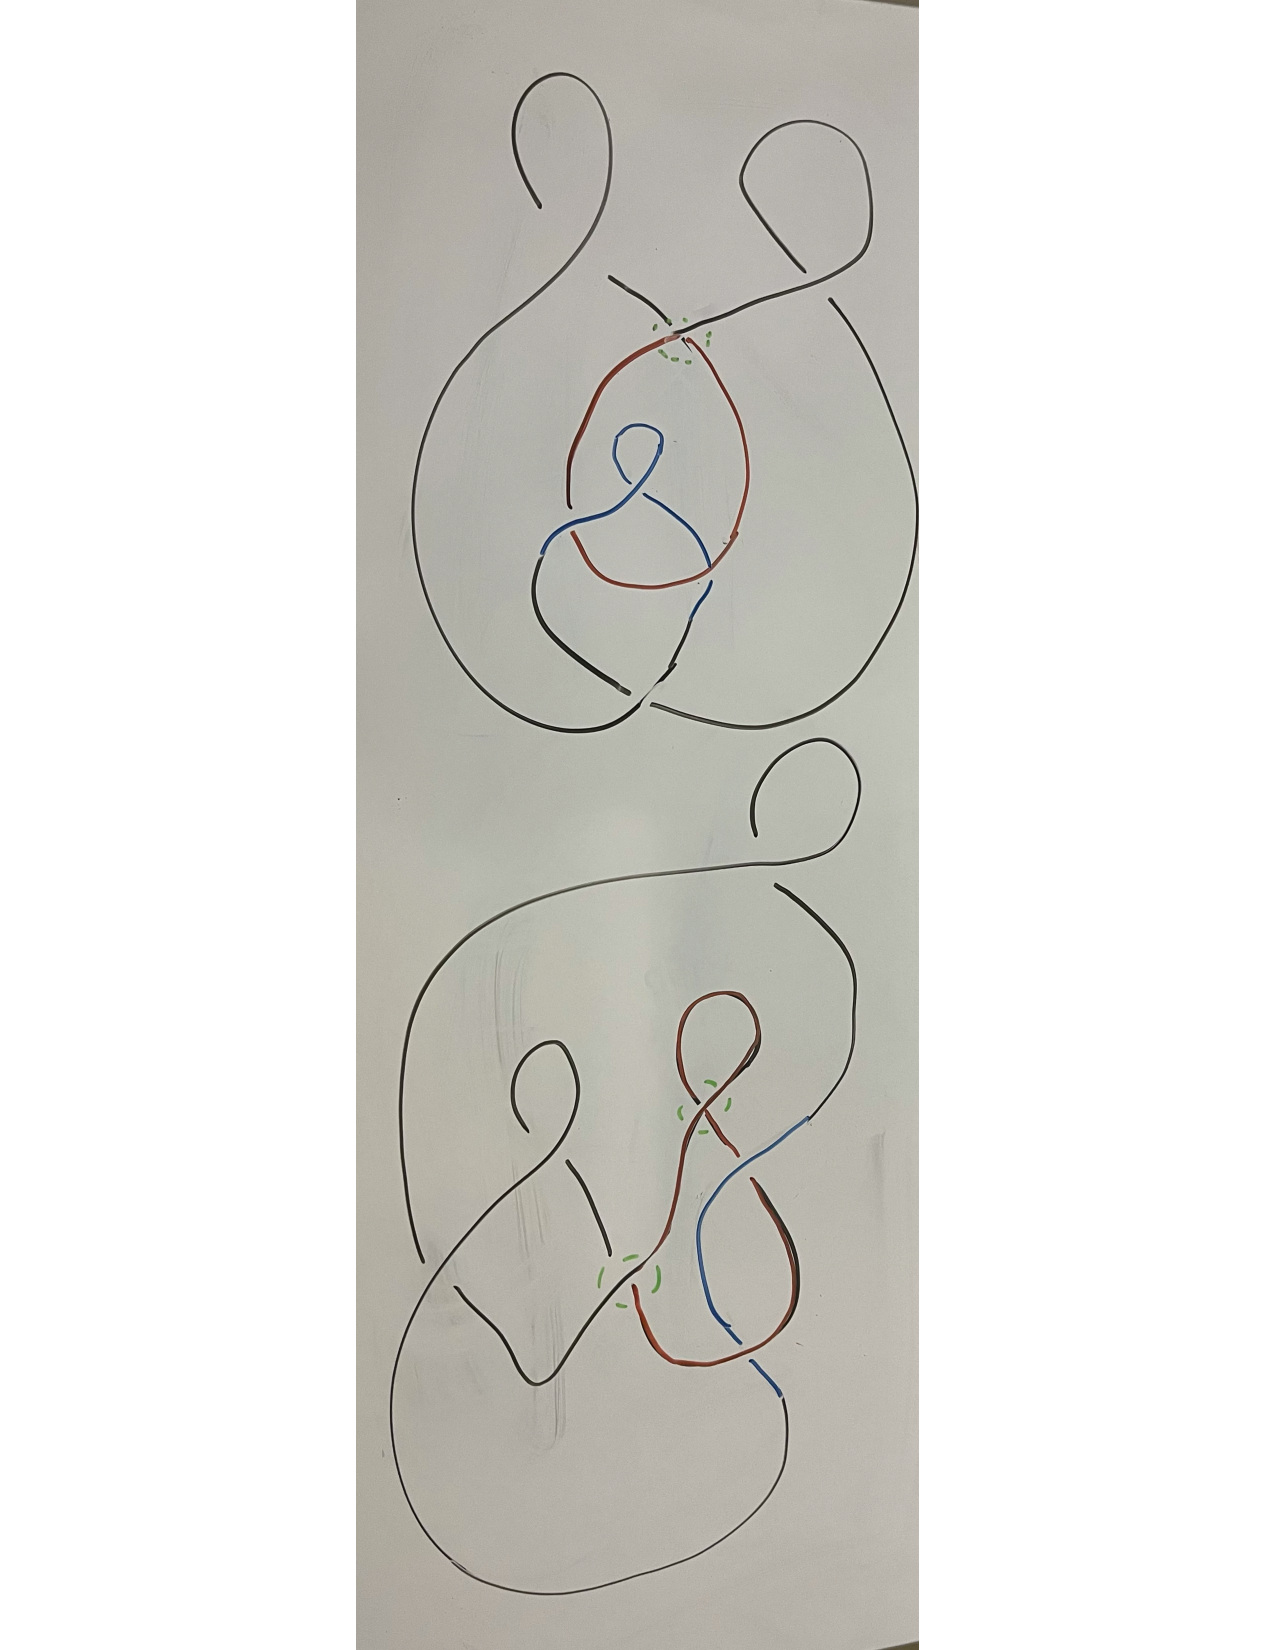
\includegraphics[angle=-90,width=\linewidth]{Journals/IMG_3518.pdf}

   
    \label{fig:mathematica}
\end{figure}






Possible future idea: what if we consider all possible augmentations when considering what is trapped (not every bar can be identified with a disk/set of disks, but perhaps we can restrict to when this is true and think about then)

\end{document}